\documentclass{beamer}

\usetheme{bjeldbak}

\title
{A short introduction to SVA and RBDyn}
\author
{Joris Vaillant}
\institute{LIRMM}{}
\date{Thursday 4 2014}
\subject{Spatial Vector Algebra, Rigid Body Physics}

\usepackage{listings}
\usepackage{graphicx}      % include this line if your document contains figures
\usepackage{amsmath} % assumes amsmath package installed
\usepackage{amsfonts} %% pour mathbb
\usepackage{upquote}

% vim: set fileencoding=utf8 :

\newcommand{\euclidspace}[1]{E^{#1}}
\newcommand{\motionspace}[1]{M^{#1}}
\newcommand{\forcespace}[1]{F^{#1}}

\newcommand{\motionvec}{\mathbf{m}}
\newcommand{\motionvecHat}{\hat{\motionvec}}
\newcommand{\motionvecOrigin}[1]{\motionvec_{#1}}
\newcommand{\motionvecHatOrigin}[1]{\motionvecHat_{#1}}

\newcommand{\motionvecDot}{\dot{\motionvec}}
\newcommand{\motionvecDotHat}{\dot{\motionvecHat}}

\newcommand{\motionvecFrame}[1]{{^{#1}\mathbf{m}}}
\newcommand{\motionvecHatFrame}[1]{{^{#1}\hat{\motionvec}}}

\newcommand{\velocityvec}{\mathbf{v}}
\newcommand{\velocityvecHat}{\hat{\velocityvec}}
\newcommand{\velocityvecOrigin}[1]{\velocityvec_{#1}}
\newcommand{\velocityvecHatOrigin}[1]{\velocityvecHat_{#1}}

\newcommand{\velocityvecDot}{\dot{\velocityvec}}
\newcommand{\velocityvecDotHat}{\dot{\velocityvecHat}}
\newcommand{\velocityvecDotOrigin}[1]{\dot{\velocityvecHat}_{#1}}
\newcommand{\velocityvecDotHatOrigin}[1]{\dot{\velocityvecHat}_{#1}}

\newcommand{\accelvec}{\mathbf{a}}
\newcommand{\accelvecHat}{\hat{\accelvec}}
\newcommand{\accelvecOrigin}[1]{\accelvec_{#1}}
\newcommand{\accelvecHatOrigin}[1]{\accelvecHat_{#1}}

\newcommand{\forcevec}{\mathbf{f}}
\newcommand{\forcevecHat}{\hat{\forcevec}}
\newcommand{\forcevecOrigin}[1]{\forcevec_{#1}}
\newcommand{\forcevecHatOrigin}[1]{\forcevecHat_{#1}}

\newcommand{\forcevecDot}{\dot{\forcevec}}
\newcommand{\forcevecDotHat}{\dot{\forcevecHat}}

\newcommand{\forcevecFrame}[1]{{^{#1}\mathbf{f}}}
\newcommand{\forcevecHatFrame}[1]{{^{#1}\hat{\forcevec}}}

\newcommand{\coord}[3]{{^#2\! #3\! _#1}}
\newcommand{\coordM}[4]{{^#2\! #3\! {_{#1}^{#4}}}}
\newcommand{\coordDual}[3]{{}^#2\! {#3}^{*}_{\! #1}}
\newcommand{\coordTrans}[3]{{}^#2\! {#3}^{T}_{\! #1}}
\newcommand{\coordInv}[3]{{}^#2\! {#3}^{-1}_{\! #1}}

\newcommand{\utransform}{X}
\newcommand{\transform}[2]{\coord{#1}{#2}{\utransform}}
\newcommand{\transformDual}[2]{\coordDual{#1}{#2}{\utransform}}
\newcommand{\transformTrans}[2]{\coordTrans{#1}{#2}{\utransform}}
\newcommand{\transformInv}[2]{\coordInv{#1}{#2}{\utransform}}
\newcommand{\transformM}[3]{\coordM{#1}{#2}{\utransform}{#3}}

\newcommand{\urotation}{E}
\newcommand{\rotation}[2]{\coord{#1}{#2}{\urotation}}
\newcommand{\rotationM}[3]{\coordM{#1}{#2}{\urotation}{#3}}

\newcommand{\utranslation}{r}
\newcommand{\translation}[2]{\coord{#1}{#2}{\utranslation}}
\newcommand{\translationM}[3]{\coordM{#1}{#2}{\utranslation}{#3}}

\newcommand{\inertia}{\mathbf{I}}
\newcommand{\inertiaBar}{\bar{\inertia}}
\newcommand{\inertiaBarOrigin}[1]{\inertiaBar_{#1}}

\newcommand{\momentum}{\mathbf{h}}
\newcommand{\momentumHat}{\hat{\momentum}}

\newcommand{\bodycom}{\mathbf{c}}
\newcommand{\mass}{\mathbf{m}}


\definecolor{listinggray}{gray}{0.9}
\definecolor{lbcolor}{rgb}{0.9,0.9,0.9}
\lstset{
backgroundcolor=\color{lbcolor},
	tabsize=2,
	%   rulecolor=,
	language=C++,
	basicstyle=\scriptsize,
	upquote=true,
	aboveskip={0.5\baselineskip},
	columns=fixed,
	showstringspaces=false,
	extendedchars=false,
	breaklines=true,
	prebreak = \raisebox{0ex}[0ex][0ex]{\ensuremath{\hookleftarrow}},
	frame=single,
	showtabs=false,
	showspaces=false,
	showstringspaces=false,
	identifierstyle=\ttfamily,
	keywordstyle=\color[rgb]{0,0,1},
	commentstyle=\color[rgb]{0.026,0.512,0.095},
	stringstyle=\color[rgb]{0.627,0.126,0.941},
	numberstyle=\color[rgb]{0.205, 0.142, 0.73},
	%        \lstdefinestyle{C++}{language=C++,style=numbers}’.
}


\begin{document}
\frame{\titlepage}

\begin{frame}
	\frametitle{Table of Contents}
	\tableofcontents
\end{frame}


\section{Spatial Vector Algebra}
\begin{frame}
\frametitle{Spatial Vector Algebra}
\framesubtitle{What is it ?}
Spatial vector algebra is a concise vector notation for describing rigid−body velocity,
acceleration, inertia, etc., using 6D vectors and tensors.
\begin{itemize}
	\item fewer quantities
	\item fewer equations
	\item less effort
	\item fewer mistakes
\end{itemize}
\end{frame}


\begin{frame}
\frametitle{Spatial Vector Algebra}
\framesubtitle{Spatial vector spaces}
There is 2 vector spaces:
\begin{itemize}
	\item $ \motionspace{6} $ - motion vector (velocity, acceleration, ...)
	\item $ \forcespace{6} $ - force vector (momentum, force, ...)
\end{itemize}
\end{frame}


\begin{frame}
\frametitle{Spatial Vector Algebra}
\framesubtitle{Spatial velocity vector}
The spatial velocity of a body computed at the point $ O $ is:
\begin{subequations}
	$$
	\velocityvecHatOrigin{O} = \begin{bmatrix} w_x \\ w_y \\ w_z \\ v_{Ox} \\ v_{Oy} \\ v_{Oz} \end{bmatrix} = \begin{bmatrix} w \\ v_O \end{bmatrix}
	$$
	$$
	\velocityvecHatOrigin{O} \in \motionspace{6}
	$$
\end{subequations}
With the angular velocity:
$ w = \begin{bmatrix} w_x\ w_y\ w_z \end{bmatrix}^T $\\
And the linear velocity at O:
$ v_O = \begin{bmatrix} v_{Ox}\ v_{Oy}\ v_{Oz} \end{bmatrix}^T $
\end{frame}


\begin{frame}
\frametitle{Spatial Vector Algebra}
\framesubtitle{Spatial acceleration vector}
The spatial acceleration of a body computed at the point $ O $ is:
\begin{subequations}
	$$
	\accelvecHatOrigin{O} = \velocityvecDotHatOrigin{O} = \begin{bmatrix} \dot{w} \\ \dot{v}_O \end{bmatrix}
	$$
	$$
	\accelvecHatOrigin{O} \in \motionspace{6}
	$$
\end{subequations}
Beware that $ \dot{v}_O $ state for tangential acceleration and normal acceleration.
If we define $ r_O $ the body O point coordinate at time $ t $, $ \dot{r}_O $ his derivative and $ \ddot{r}_O $ his acceleration, then $ \dot{v}_O = \ddot{r}_O - w \times \dot{r}_O $ 

\hfill \\
We will use $ \motionvecHat $ to describe a generic motion vector.
\end{frame}


\begin{frame}
\frametitle{Spatial Vector Algebra}
\framesubtitle{Spatial force vector}
The spatial force of a point $ O $ of a body is:
\begin{subequations}
	$$
	\forcevecHatOrigin{O} = \begin{bmatrix} n_{Ox} \\ n_{Oy} \\ n_{Oz} \\ f_x \\ f_y \\ f_z \end{bmatrix} = \begin{bmatrix} n_O \\ f \end{bmatrix}
	$$
	$$
	\forcevecHatOrigin{O} \in \forcespace{6}
	$$
\end{subequations}
With the torque at point O:
$ n_O = \begin{bmatrix} n_{Ox}\ n_{Oy}\ n_{Oz} \end{bmatrix}^T $\\
			And the force:	
$ f = \begin{bmatrix} f_x\ f_y\ f_z \end{bmatrix}^T $.
\end{frame}


\begin{frame}
\frametitle{Spatial Vector Algebra}
\framesubtitle{Spatial transformations}
The motion vector transformation from the frame A to B is written:
$$
\transform{A}{B} = \begin{bmatrix} \rotation{A}{B} & 0 \\ -\rotation{A}{B} \translation{A}{B} \times & \rotation{A}{B} \end{bmatrix}
$$
With $ \rotation{A}{B} \in \mathbb{R}^{3{\times}3} $ and $ \translation{A}{B} \in \mathbb{R}^{3} $ the A to B anti trigonometric rotation matrix and translation vector.

\hfill \\
To apply the same transformation to a force vector, we must use the dual transform:
$$
\transformDual{A}{B} = (\transformInv{A}{B})^T
$$
\end{frame}


\begin{frame}
\frametitle{Spatial Vector Algebra}
\framesubtitle{Transformations example}
Transform a motion vector in A frame $ \motionvecHatFrame{A} $ to B frame $ \motionvecHatFrame{B} $:
$$
\motionvecHatFrame{B} = \transform{A}{B} \motionvecHatFrame{A}
$$

Transform a force vector in A frame $ \forcevecHatFrame{A} $ to B frame $ \forcevecHatFrame{B} $:
$$
\forcevecHatFrame{B} = \transformDual{A}{B} \forcevecHatFrame{A}
$$

Find the transformation between A and C frame:
$$
\transform{A}{C} = \transform{B}{C}\transform{A}{B}
$$
\end{frame}


\begin{frame}
\frametitle{Spatial Vector Algebra}
\framesubtitle{Spatial rigid body inertia}
The spatial inertia at the origin O of a body is:
$$
\inertia = \begin{bmatrix} \inertiaBarOrigin{O} & \mass \bodycom \times \\ -\mass \bodycom \times & \mass1 \end{bmatrix}
$$
With $ \inertiaBarOrigin{O} $ is the body inertia matrix at his origin O, $ \mass $ the body mass and $ \bodycom = \translation{O}{{CoM}} $ the translation between the body origin and his center of mass.

\hfill \\
This matrix allow to transform a $ \motionspace{6} $ in a $ \forcespace{6} $.
\end{frame}


\begin{frame}
\frametitle{Spatial Vector Algebra}
\framesubtitle{Spatial inertia use}
Transform an acceleration to a force:
$$
\forcevecHat = \inertia \accelvecHat
$$
A velocity to a spatial momentum:
$$
\momentumHat = \inertia \velocityvecHat
$$
Merge body $ b_2 $ inertia into body $ b_1 $ inertia:
$$
{}^{b_1+b_2}\inertia = {}^{b_1}\inertia + \transform{{b_2}}{{b_1}} {}^{b_2}\inertia\transformInv{{b_2}}{{b_1}}
$$
\end{frame}
\section{SpaceVecAlg Library}

\begin{frame}
\frametitle{SpaceVecAlg}
\framesubtitle{What's in ?}
\begin{itemize}
	\item Featherstone Spatial Vector Algebra C++11 implementation
	\item Header only
	\item Use Eigen3 as linear algebra library
	\item Python binding
\end{itemize}
\end{frame}


\begin{frame}[fragile]
\frametitle{SpaceVecAlg}
\framesubtitle{MotionVec}
MotionVec is the Spatial Motion Vector implementation:
\begin{lstlisting}[language=C++]
	Eigen::Vector3d w, v;

	sva::MotionVecd mv1(w, v); // constructor
	w == mv1.angular(); // angular getter
	v == mv1.linear(); // linear getter

	sva::MotionVecd mv2;
	mv1 + mv2; // addition
	mv1 - mv2; // subtraction
	10.*mv1; // scalar multiplication
\end{lstlisting}
\end{frame}


\begin{frame}[fragile]
\frametitle{SpaceVecAlg}
\framesubtitle{ForceVec}
ForceVec is the Spatial Force Vector implementation:
\begin{lstlisting}[language=C++]
	Eigen::Vector3d t, f;

	sva::ForceVecd fv1(t, f); // constructor
	t == mv1.couple(); // couple getter
	f == mv1.force(); // force getter

	sva::ForceVecd fv2;
	fv1 + fv2; // addition
	fv1 - fv2; // subtraction
	10.*fv1; // scalar multiplication
\end{lstlisting}
\end{frame}


\begin{frame}[fragile]
\frametitle{SpaceVecAlg}
\framesubtitle{RBInertia}
RBInertia is the Spatial Rigid Body Inertia implementation:
\begin{lstlisting}[language=C++]
	Eigen::Vector3d com; // orgin to CoM translation
	double mass; // rigid body mass
	Eigen::Vector3d h = com*mass; // first moment of mass
	Eigen::Matrix3d I; // rigid body inertia at origin

	sva::RBInertiad rbi1(mass, h, I); // constructor
	mass == rbi1.mass(); // mass getter
	h == rbi1.momentum(); // momentum getter
	I == rbi1.inertia(); // inertia getter

	sva::RBInertiad rbi2(mass, h, I); // constructor
	rbi1 + rbi2; // addition
	rbi1 - rbi2; // subtraction
	10.*rbi1; // scalar multiplication (only on mass and h)

	sva::MotionVecd mv;
	sva::ForceVecd fv = rbi1*mv; // motion space to force space
\end{lstlisting}
\end{frame}


\begin{frame}[fragile]
\frametitle{SpaceVecAlg}
\framesubtitle{PTransform}
PTransform is the Spatial Transformation implementation:
\begin{lstlisting}[language=C++]
	Eigen::Matrix3d E; // rotation
	Eigen::Quaterniond q; // rotation
	Eigen::Vector3d r; // translation

	sva::PTransformd X1(E,r); // constructors
	sva::PTransformd X2(q,r); // quaternion -> matrix
	sva::PTransformd X3 = sva::PTransformd::Identity();
	E == X1.rotation(); // rotation getter
	r == X1.translation(); // translation getter

	// inverse function
	E.transpose() == X1.inv().rotation();
	-E*r == X1.inv().translation();
\end{lstlisting}
\end{frame}
\begin{frame}[fragile]
\frametitle{SpaceVecAlg}
\framesubtitle{PTransform}
\begin{lstlisting}[language=C++]
	// motion vector transform and inverse transform
	sva::MotionVecd mv;
	sva::MotionVecd mv1 = X1*mv;
	mv == X1.invMul(mv1);

	// force vector transform and inverse transform
	sva::ForceVecd fv;
	sva::ForceVecd fv1 = X.dualMul(fv);
	fv == X.transMul(fv1);

	// inertia transform and inverse transform
	sva::RBInertiad rbi;
	sva::RBinertia rbi1 = X.dualMul(rbi);
	rbi == X.transMul(rbi1);
\end{lstlisting}
\end{frame}


\begin{frame}[fragile]
\frametitle{SpaceVecAlg}
\framesubtitle{Utilities}
Some useful functions:
\begin{lstlisting}[language=C++]
	// Anti trigonometric rotation around 1 axis
	double theta;
	Eigen::Matrix3d Ex = sva::RotX(theta); // X rotation
	Eigen::Matrix3d Ey = sva::RotY(theta); // Y rotation
	Eigen::Matrix3d Ez = sva::RotZ(theta); // Z rotation

	// 3d projection of rotation error
	// x, y, z rotation to go from Ex to Ey
	Eigen::Vector3d sva::rotationError(Ex, Ey);

	// compute inertia at origin from inertia at CoM
	Eigen::Matrix3d IatCoM, IatO;
	Eigen::Matrix3d E; // rotation from origin to com frame
	Eigen::Vector3d com; // translation from origin to com
	double mass;
	IatO = inertiaToOrigin(IatCoM, mass, com, E);
\end{lstlisting}
\end{frame}

\section{Rigid Body System}

\begin{frame}
\frametitle{Rigid Body System}
\framesubtitle{Description}
A rigid body system is composed of a set of body linked by joint.
There is many kind of rigid body system:
\begin{itemize}
	\item Kinematic chain
	\item Kinematic tree
	\item Closed loop kinematic tree
\end{itemize}
We will focus on kinematic tree.
\end{frame}
\begin{frame}
\frametitle{Rigid Body System}
\framesubtitle{Body}
A kinematic tree contains $ N_B $ body.

\hfill \\
A body $ i \in \{1, \cdots, N_B\} $ is associated to an inertia $ I_i $.

\hfill \\
The parent body index of a body $ i \in \{1, \cdots, N_B\} $ is give by the $ \lambda $ array.
\end{frame}
\begin{frame}
\frametitle{Rigid Body System}
\framesubtitle{Joint}
A kinematic tree contains $ N_B $ joint.

\hfill \\
A joint $ i \in \{1, \cdots, N_B\} $ support the body $ i $.

\hfill \\
$ jtype(i) $ identify the joint $ i \in \{1, \cdots, N_B\} $ type.

\hfill \\
			The transformation $ \utransform_{Ti} $ identify the joint $ i \in \{1, \cdots, N_B\} $
static transformation between his parent body $ \lambda(i) $ and the joint $ i $ origin.
\end{frame}
\begin{frame}
\frametitle{Rigid Body System}
\framesubtitle{Joint type}
Each joint are characterized by a type $ jtype $.

\hfill \\
This type allow us to size of his general position vector $ \mathbf{q}_J $ and the size
of his general velocity vector $ \mathbf{\alpha}_J $.

\hfill \\
With the $ jtype $, $ \mathbf{q}_J $ and $ \mathbf{\alpha}_J $ we are able to compute the joint
transformation $ \utransform_J $ , motion subspace matrix $ \mathbf{S} $ and
the joint velocity $ \velocityvec_J $:
$$
[\utransform_J, \mathbf{S}, \velocityvec_J] = jcalc(jtype, \mathbf{q}_J, \mathbf{\alpha}_J)
$$

We can compute the joint velocity with the motion subspace matrix and
the general velocity vector $ \velocityvec_J = \mathbf{S}\mathbf{\alpha}_J $.
That allow to compute the kinematics tree Jacobian really easily.
\end{frame}
\begin{frame}
\frametitle{Rigid Body System}
\framesubtitle{Illustration of a kinematics tree}
\begin{columns}[T]
	\begin{column}[T]{5cm}
		\begin{figure}
			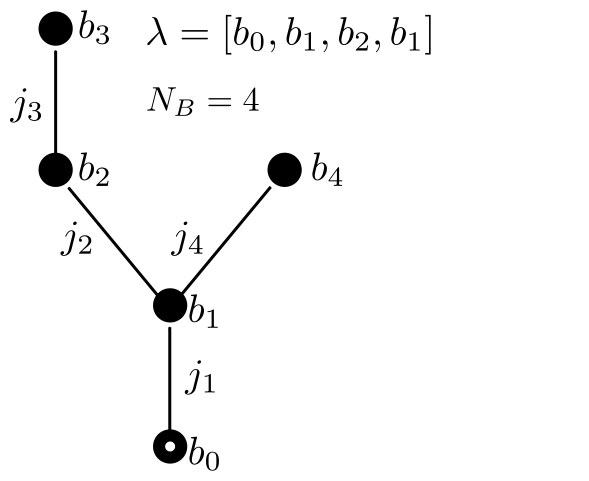
\includegraphics[height=5cm]{img/robot1_graph.pdf}
			\caption{Connectivity graph of a rigid body system}
		\end{figure}
	\end{column}
	\begin{column}[T]{5cm}
		\begin{figure}
			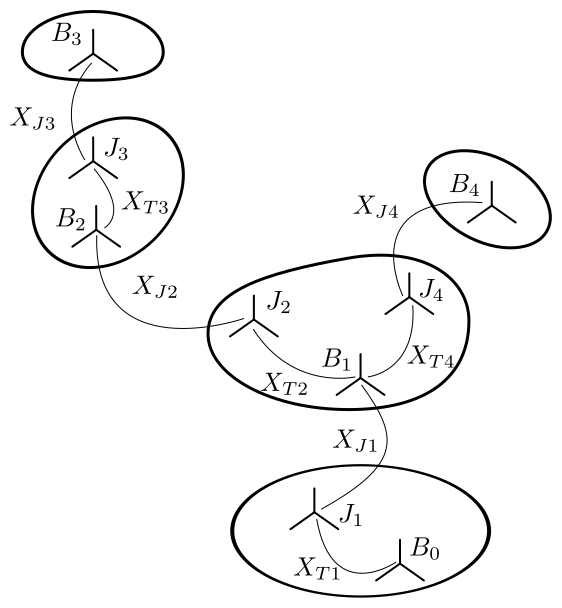
\includegraphics[height=5cm]{img/robot1_illu.pdf}
			\caption{Geometric model of a rigid body system}
		\end{figure}
	\end{column}
	 \end{columns}
\end{frame}



\section{RBDyn Library}
\begin{frame}
\frametitle{RBDyn}
\framesubtitle{Description}
\begin{itemize}
	\item Kinematics tree Kinematics and Dynamics algorithm C++11 implementation
	\item Use Eigen3 and SpaceVecAlg library
	\item Free, Spherical, Planar, Cylindrical, Revolute, Prismatic joint support
	\item Translation, Rotation, Vector, CoM, Momentum Jacobian computation
	\item Inverse Dynamics, Forward Dynamics
	\item Inverse Dynamic Identification Model (IDIM)
	\item Kinematics tree body merging/filtering
	\item Kinematics tree base selection
	\item Python binding
\end{itemize}
\end{frame}

\begin{frame}[fragile]
\frametitle{RBDyn}
\framesubtitle{Body}
A body is constituted of a spatial inertia, and is identified by an unique id and name:
\begin{lstlisting}[language=C++]
	sva::RBInertiad rbi; // body inertia
	Eigen::Vector3d r_com;
	Eigen::Matrix3d I;
	double mass;
	int id;
	std::string name;

	// constructors
	rbd::Body b1(rbi, id, name);
	rbd::Body b2(mass, r_com, I, id, name);

	rbi == b1.inertia(); // inertia getter
	id == b1.id(); // id getter
	name == bi1.name(); // name getter
\end{lstlisting}
\end{frame}

	\begin{frame}[fragile]
	\frametitle{RBDyn}
	\framesubtitle{Joint}
	A joint is constituted of a type, an optional axis, a direction and like the body is identified by an
	unique id and name:
	\begin{lstlisting}[language=C++]
		Joint::Type type; // Rev, Prism, Spherical, Planar, Cylindrical, Free and Fixed
		Eigen::Vector3d axis; // For Rev, Prism and Cylindrical
		bool direction; // true forward, false backward
		int id;
		std::string name;

		// constructors
		rbd::Joint j1(type, axis, direction, id, name);
		rbd::Joint j2(type, direction, id, name);

		type == j1.type(); // type getter
		direction == j1.forward(); // direction getter
		id == j1.id(); // id getter
		name == j1.name(); // name gette
	\end{lstlisting}
\end{frame}
	\begin{frame}[fragile]
	\frametitle{RBDyn}
	\framesubtitle{Joint}
	\begin{lstlisting}[language=C++]
		j1.params(); // q vector size
		j1.dof(); // alpha vector size

		j1.motionSubsace(); // motion subspace matrix (S)

		// transformation and velocity
		std::vector<double> q(j.params()), alpha(j.dof()),
												alphaDot(j.dof());
		j1.pose(q); // X_j transformation matrix
		j1.motion(alpha); // v_j motion vector
		j1.tanAccel(alphaDot); // tangential acceleration

		// initialization
		j1.zeroParam(); // identity q vector
		j1.zeroDof(); // identity alpha, alphaDot vector
	\end{lstlisting}
\end{frame}

	\begin{frame}[fragile]
	\frametitle{RBDyn}
	\framesubtitle{MultiBodyGraph}
	A non oriented graph that model the robot:
	\begin{lstlisting}[language=C++]
		sva::RBInertiad rbi;
		rbd::Body b1(rbi, 1, "b1"), b2(rbi, 2, "b2"),
							b3(rbi, 3, "b3");
		rbd::Joint j1(rbd::Joint::Rev, Eigen::Vector3d::UnitX,
									true, 1, "j1");
		rbd::Joint j2(rbd::Joint::Spherical, true, 2, "j2");
		sva::PTransformd X_12, X_13;
		sva::PTransformd I(sva::PTransformd::Identity());

		rbd::MultiBodyGraph mbg; // constructor
		mbg.addBody(b1);mbg.addBody(b2);mbg.addBody(b3);
		mbg.addJoint(j12);mbg.addJoint(j13);

		// link body b1 to body b2 with joint j1 and static transform X_12
		mbg.linkBodies(1, X_12, 2, I, 1);
		// link body b1 to body b3 with joint j2 and static transform X_13
		mbg.linkBodies(1, X_13, 3, I, 2);
	\end{lstlisting}
\end{frame}
	\begin{frame}[fragile]
	\frametitle{RBDyn}
	\framesubtitle{MultiBodyGraph}
	\begin{lstlisting}[language=C++]
		// create a multibody with b1 as fixed root body
		rbd::MultiBody mb1 = mbg.makeMultiBody(1, rbd::Joint::Fixed);

		sva::PTransformd X_O_j0, X_b0_j0;
		// multibody with b2 as planar base 
		// X_O_j0 is the transform from the world to the planar joint
		// X_b0_j0 is the transform from b2 to the joint (X_T)
		rbd::MultiBody mb2 = mbg.makeMultiBody(2, rbd::Joint::Planar, X_O_j0, X_b0_j0);

		// remove a joint and his subtree
		mbg.removeJoint(...);

		// merge a sub tree in one body
		mbg.mergeSubBodies(...);

		// compute bodies transformation to them origin
		mbg.bodiesBaseTransform(...);
	\end{lstlisting}
\end{frame}
	\begin{frame}
	\frametitle{RBDyn}
	\framesubtitle{MultiBodyGraph illustration}
	\begin{columns}[T]
		\begin{column}[T]{5cm}
			\begin{figure}
				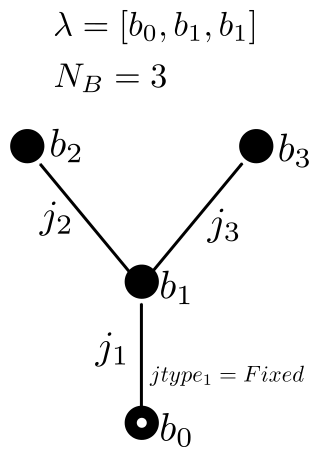
\includegraphics[height=5cm]{img/robot2_graph.pdf}
				\caption{mb1 connectivity graph}
			\end{figure}
		\end{column}
		\begin{column}[T]{5cm}
			\begin{figure}
				\includegraphics[height=5cm]{img/robot3_graph.pdf}
				\caption{mb2 connectivity graph}
			\end{figure}
		\end{column}
		 \end{columns}
\end{frame}

\begin{frame}[fragile]
	\frametitle{RBDyn}
	\framesubtitle{MultiBody}
	Kinematics tree implementation:
	\begin{lstlisting}[language=C++]
		mb1.nrBodies() == 3; // Body number
		mb1.nrJoints() == 3; // Joint number

		mb1.bodies(); // bodies array
		mb1.joints(); // joints array

		// body that pred/succ a joint
		mb1.predecessors();
		mb1.successors();
		mb1.parents(); // lambda
		mb1.transfroms(); // X_T array

		// body/joint index by id
		mb1.bodyIndexById(id);
		mb1.jointIndexById(id);

		mb1.bodyIndexById(1) != mb2.bodyIndexById(1);
	\end{lstlisting}
\end{frame}
\begin{frame}[fragile]
	\frametitle{RBDyn}
	\framesubtitle{MultiBody}
	\begin{lstlisting}[language=C++]
		//                     Spherical   Rev   Fixed
		mb1.nrParams() == 5; //   4         1      0
		mb1.nrDof() == 4;    //   3         1      0

		//                     Spherical   Rev   Planar
		mb2.nrParams() == 8; //   4         1      3
		mb2.nrDof() == 7;    //   3         1      3

		mb1.jointPosInParam(index) // joint position in flat q
		mb1.jointPosInDof(index) // joint position in flat alpha
	\end{lstlisting}
\end{frame}

\begin{frame}[fragile]
	\frametitle{RBDyn}
	\framesubtitle{MultiBodyConfig}
	Configuration of a multi body is separated from his model:
	\begin{lstlisting}[language=C++]
		rbd::MultiBodyConfig mbc1(mb1);
		mbc1.zero(mb1); // set q, alpha, alphaD and jointTorque to 0

		// indexed by joint
		// std::vector<std::vector<double>>
		mbc1.q; // q generalized position vector
		mbc1.alpha; // alpha generalized velocity vector
		mbc1.alphaD; // q generalized acceleration vector
		mbc1.jointTorque; // joint torque
		mbc.S; // motion subspace matrix

		// indexed by body
		mbc1.force; // Force apply on each body
		mbc1.bodyPosW; // Body transformation in world coord
		mbc1.bodyVelW; // Body velocity in world coord
		mbc1.bodyVelB; // Body velocity in body coord

		mbc.gravity; // gravity apply on the system
		...
	\end{lstlisting}
\end{frame}


\begin{frame}[fragile]
	\frametitle{RBDyn}
	\framesubtitle{MultiBodyConfig usefull functions}
	\begin{lstlisting}[language=C++]
		// convert q, alpha, alphaD and force vector
		// from mbc1 to mbc2
		// mbc1 and mbc2 must come from the same mbg
		// don't convert root joint
		rbd::ConfigConverter(mbc1, mbc2);

		Eigen::VectorXd q;
		// to and from flat vector
		paramToVector(mbc.q, q);
		vectorToParam(q, mbc.q);
	\end{lstlisting}
\end{frame}

\begin{frame}[fragile]
	\frametitle{RBDyn}
	\framesubtitle{Algorithm}
	\begin{lstlisting}[language=C++]
		// q -> bodyPosW
		rbd::forwardKinematics(mb1, mbc1);

		// alpha, FK -> bodyVelW, bodyVelB, S
		rbd::forwardVelocity(mb1, mbc1);

		// alphaD, gravity, FV -> jointTorque
		rbd::InverseDynamics id(mb1);
		id.inverseDynamics(mb1, mbc1);

		// jointTorque, FV -> alphaD, H, C
		rbd::ForwardDynamics fd(mb1);
		fd.forwardDynamics(mb1, mbc1);

		// FK -> CoM
		rbd::computeCoM(mb1, mbc1);

		// FV -> CoM speed
		rbd::computeCoMVelocity(mb1, mbc1);
	\end{lstlisting}
\end{frame}

\begin{frame}[fragile]
	\frametitle{RBDyn}
	\framesubtitle{Jacobian}
	Like the 6D vector, the rotation part of the Jacobian is the 3 first row and the translation part is the 3 last row.
	\begin{lstlisting}[language=C++]
		Eigen::Vector3d bodyPoint;
		rbd::Jacobian jac(mb1, bodyId, bodyPoint);
		// 6D bodyId world coord jacobian at bodyPoint
		jac.jacobian(mb1, mbc1);
		// bodyId coordinate
		jac.bodyJacobian(mb1, mbc1);

		Eigen::Vector3d vec;
		// 3D world coord jacobian of a vector in bodyId
		jac.vectorJacobian(mb1, mbc1, vec);
		// bodyId coordinate
		jac.bodyVectorJacobian(mb1, mbc1, vec);

		// translate a jacobian to a specific point
		jac.translateJacobian(...);

		// project a jacobian in the robot parameter vector
		jac.fullJacobian(...);
	\end{lstlisting}
\end{frame}

\begin{frame}
	\frametitle{RBDyn}
	\framesubtitle{Other stuff}
	\begin{itemize}
		\item Jacobian time derivative $ \dot{J} $ computation
		\item Jacobian normal acceleration vector $ \dot{J}\dot{\mathbf{q}} $ computation
		\item CoM Jacobian
		\item Centroidal Momentum Matrix $ A_g $ and $ \dot{A}_g $
		\item Centroidal ZMP
		\item Euler integration
	\end{itemize}
\end{frame}

\begin{frame}[fragile]
	\frametitle{RBDyn}
	\framesubtitle{Example: problem}
	We want to write a function that given a kinematics tree
	and the body id of $ b_1 $ and $ b_2 $, return true if it's possible that the two bodies enter in self collision.
	\\ \hfill

	To solve this problem we have the following structure and function:
	\begin{lstlisting}[language=C++]
		// collision data of a robot
		struct CollisionData;

		// return true if b1 and b2 are in collision
		bool isInCollision(const sva::PTransformd& Xb1,
											 const sva::PTransformd& Xb2,
											 int b1Id, int b2Id,
											 const CollisionData&);
	\end{lstlisting}
	
	Let's solve this problem by using sampling.
\end{frame}
\begin{frame}[fragile]
	\frametitle{RBDyn}
	\framesubtitle{Example: sampling (1/2)}
	\begin{lstlisting}[language=C++,basicstyle=\tiny]
		bool isCollPossible(const rbd::MultiBody& mb, int b1Id, int b2Id,
												const CollisionData& cd, int N)
		{
			rbd::MultiBodyConfig mbc(mb); // create the robot configuration
			mbc.zero(mb); // init the configuration to 0
			Eigen::VectorXd q(mb.nrParams()); // create q vector as Eigen3 vector
			// take the body index from body id
			// because mbc.bodyPosW vector is ordered by index
			int b1Index = mb.bodyIndexById(b1Id);
			int b2Index = mb.bodyIndexById(b2Id);

			for(int i = 0; i < N; ++i)
			{
				randomParam(mb, q); // generate a random q vector
				rbd::vectorToParam(q, mbc.q); // fill mbc.q vector with q
				rbd::forwardKinematics(mb, mbc); // use mbc.q to compute mbc.bodyPosW
				if(isInCollision(mbc.bodyPosW[b1Index],
					 mbc.bodyPosW[b2Index],
					 b1Id, b2Id, cd))
				{
					return true;
				}
			}
			return false;
		}
	\end{lstlisting}
\end{frame}
\begin{frame}[fragile]
	\frametitle{RBDyn}
	\framesubtitle{Example: sampling (2/2)}
	\begin{lstlisting}[language=C++,basicstyle=\tiny]
		void randomParam(const rbd::MultiBody& mb, Eigen::VectorXd& q)
		{
			// fill q with random values
			q.setRandom();

			// if a joint is spherical or free there is a quaternion inside
			// so we must normalize it
			// spherical = [qw, qx, qy, qz]
			// free = [qw, qx, qy, qz, tx, ty, tz]
			for(int i = 0; i < mb.nrJoints(); ++i)
			{
				if(mb.joint(i).type() == rbd::Joint::Spherical ||
					 mb.joint(i).type() == rbd::Joint::Free)
				{
					// jointPosInParam find the joint position in the flat q vector
					q.segment(mb.jointPosInParam(i), 4).normalize();
				}
			}
		}
	\end{lstlisting}
\end{frame}

\begin{frame}
	\frametitle{RBDyn}
	\framesubtitle{Example: using Jacobian}
	OK, it's cool, we solve the problem using sampling.
	Some labs could wrote a paper about that...
	\\ \hfill

	But maybe we could find a better solution.
	\\ \hfill

	If we find $ \delta q $ that minimize the distance between $ b_1 $ and $ b_2 $
	we can find if two body can go in collision faster.
	$$
	\delta q = (J_{tr_{b_1}} - J_{tr_{b_2}})^{\#} (\translation{O}{{b_1}} - \translation{O}{{b_2}})
	$$
	Where $ \# $ state for the pseudo inverse and $ J_{tr} $ the translation Jacobian.
\end{frame}
\begin{frame}[fragile]
	\frametitle{RBDyn}
	\framesubtitle{Example: optim (1/2)}
	\begin{lstlisting}[language=C++,basicstyle=\tiny]
		bool isCollPossible(const rbd::MultiBody& mb, int b1Id, int b2Id,
												const CollisionData& cd, int N, double dt)
		{
			rbd::MultiBodyConfig mbc(mb); // create the robot configuration
			mbc.zero(mb); // init the configuration to 0
			rbd::forwardKinematics(mb, mbc); // use mbc.q to compute mbc.bodyPosW
			rbd::forwardVelocity(mb, mbc); // fill mbc.S used by Jacobian
			rbd::Jacobian jb1(mb, b1Id), jb2(mb, b2Id); // b1 and b2 jacobian
			Eigen::VectorXd alpha(mb.nrDof()); // general velocity vector
			// jacobian matrix
			Eigen::MatrixXd jMb1(3, mb.nrDof()), jMb2(3, mb.nrDof());
			Eigen::MatrixXd jMPInv(mb.nrDof(), 3);

			int b1Index = mb.bodyIndexById(b1Id);
			int b2Index = mb.bodyIndexById(b2Id);
			for(int i = 0; i < N; ++i)
			{
				// compute delta q and put it in mbc.alpha
				computeDQ(mb, mbc, alpha, b1Index, b2Index,
									jb1, jb2, jMb1, jMb2, jPInv)
				rbd::eulerIntegration(mb, mbc, dt); // q += dt*alpha
				rbd::forwardKinematics(mb, mbc);
				if(isInCollision(mbc.bodyPosW[b1Index], mbc.bodyPosW[b2Index],
					 b1Id, b2Id, cd))
				{
					return true;
				}
			}
			return false;
		}
	\end{lstlisting}
\end{frame}
\begin{frame}[fragile]
	\frametitle{RBDyn}
	\framesubtitle{Example: optim (2/2)}
	\begin{lstlisting}[language=C++,basicstyle=\tiny]
		void computeDQ(const rbd::MultiBody& mb, const rbd::MultiBodyConfig& mbc,
									 Eigen::VectorXd& alpha,
									 int b1Index, int b2Index, rbd::Jacobian& jb1,
									 rbd::Jacobian& jb2, Eigen::MatrixXd& jb1M,
									 Eigen::MatrixXd& jb2M, Eigen::MatrixXd& jPInv)
		{
			// compute the position error between b1 and b2
			Eigen::Vector3d err = mbc.bodyPosW[b1Index].translation() -
														mbc.bodyPosW[b2Index].translation();
			// compute the b1 and b2 jacobian and take back the translation part
			const auto& j1tr = jb1.jacobian(mb, mbc).block(3, 0, 3, jb1.dof());
			const auto& j2tr = jb2.jacobian(mb, mbc).block(3, 0, 3, jb2.dof());

			// project the translation jacobian into full jacobian
			jb1.fullJacobian(mb, j1tr, jb1M);
			jb2.fullJacobian(mb, j2tr, jb2M);

			// compute the position minimization jacobian
			jb1M -= jb2M;

			// compute alpha by using the jb1M pseudo inverse
			Eigen::pinv(jb1M, jPInv);
			alpha = jPinv*err;
			rbd::vectorToParam(alpha, mbc.alpha);
		}
	\end{lstlisting}
\end{frame}

\begin{frame}
	\frametitle{Next time}
	\framesubtitle{}
	We will see how to use SpaceVecAlg and RBDyn in Python with ROS.
	
	\hfill \\
	In the same time we will learn how to use Tasks library to do whole body control on an humanoid robot.

	\hfill \\
	{\centering
	Stay tuned !\par}
	\hfil \\
	{\centering
	...\par}
	\hfill \\
	{\centering
	\bf{Questions} ?\par}
\end{frame}
\end{document}

